\subsection*{Meetings for Coordination\label{sec:meetings-for-coordination}}

In an organization comprised of more than one person, meetings are necessary to facilitate coordination. The coordination accomplished by a meeting can be explicit (verbal or written), or it can be indirect through signaling (who attended the meeting, when the meeting was held, where the meeting was held, how much notice was provided). 

Not everyone understands that meetings are a vital aspect of coordination in a bureaucracy. The following sequence of scenarios illustrate the thinking some bureaucrats use.
\index{decrease surprise!anti-meeting anti-planning}
If you're already convinced of the value of meetings, see \hyperref[sec:well-run-meeting]{tips on improvement}
on page~\pageref{sec:well-run-meeting}.


\ \\
% https://graphthinking.blogspot.com/2021/07/thought-terminating-concepts-in.html
\textit{Anti-meeting view}: No plan or coordination needed; I just do what you tell me. With this approach, either I will be successful because I worked hard on what my supervisor directed, or I will fail because I was directed to do the wrong thing by my supervisor.\\
\textit{Potential response 1 by the supervisor}: I think you're smart, and I think you're capable of shaping your career. Let's work as a team to improve your effectiveness. \\
\textit{Potential response 2 by the supervisor}: Is that how you want your career to go? Do you desire autonomy and creativity?

\ \\
\textit{Anti-meeting view}: No point in making a plan or coordinating because everything changes so often. \\
\textit{Potential response by the supervisor}: But the work has an end goal, right?\\
\textit{Anti-meeting view}:  Yes, so then the plan is to get from where we are now to that end goal. Coordinate as necessary. \\
\textit{Potential response by the supervisor}: And there are no intermediary steps? Milestones?
Is it better to have no plans and just put out fires as a reaction, or to have a plan with contingencies that are subject to change? %To wait for a need for coordination?

\begin{figure}[H]
    \centering
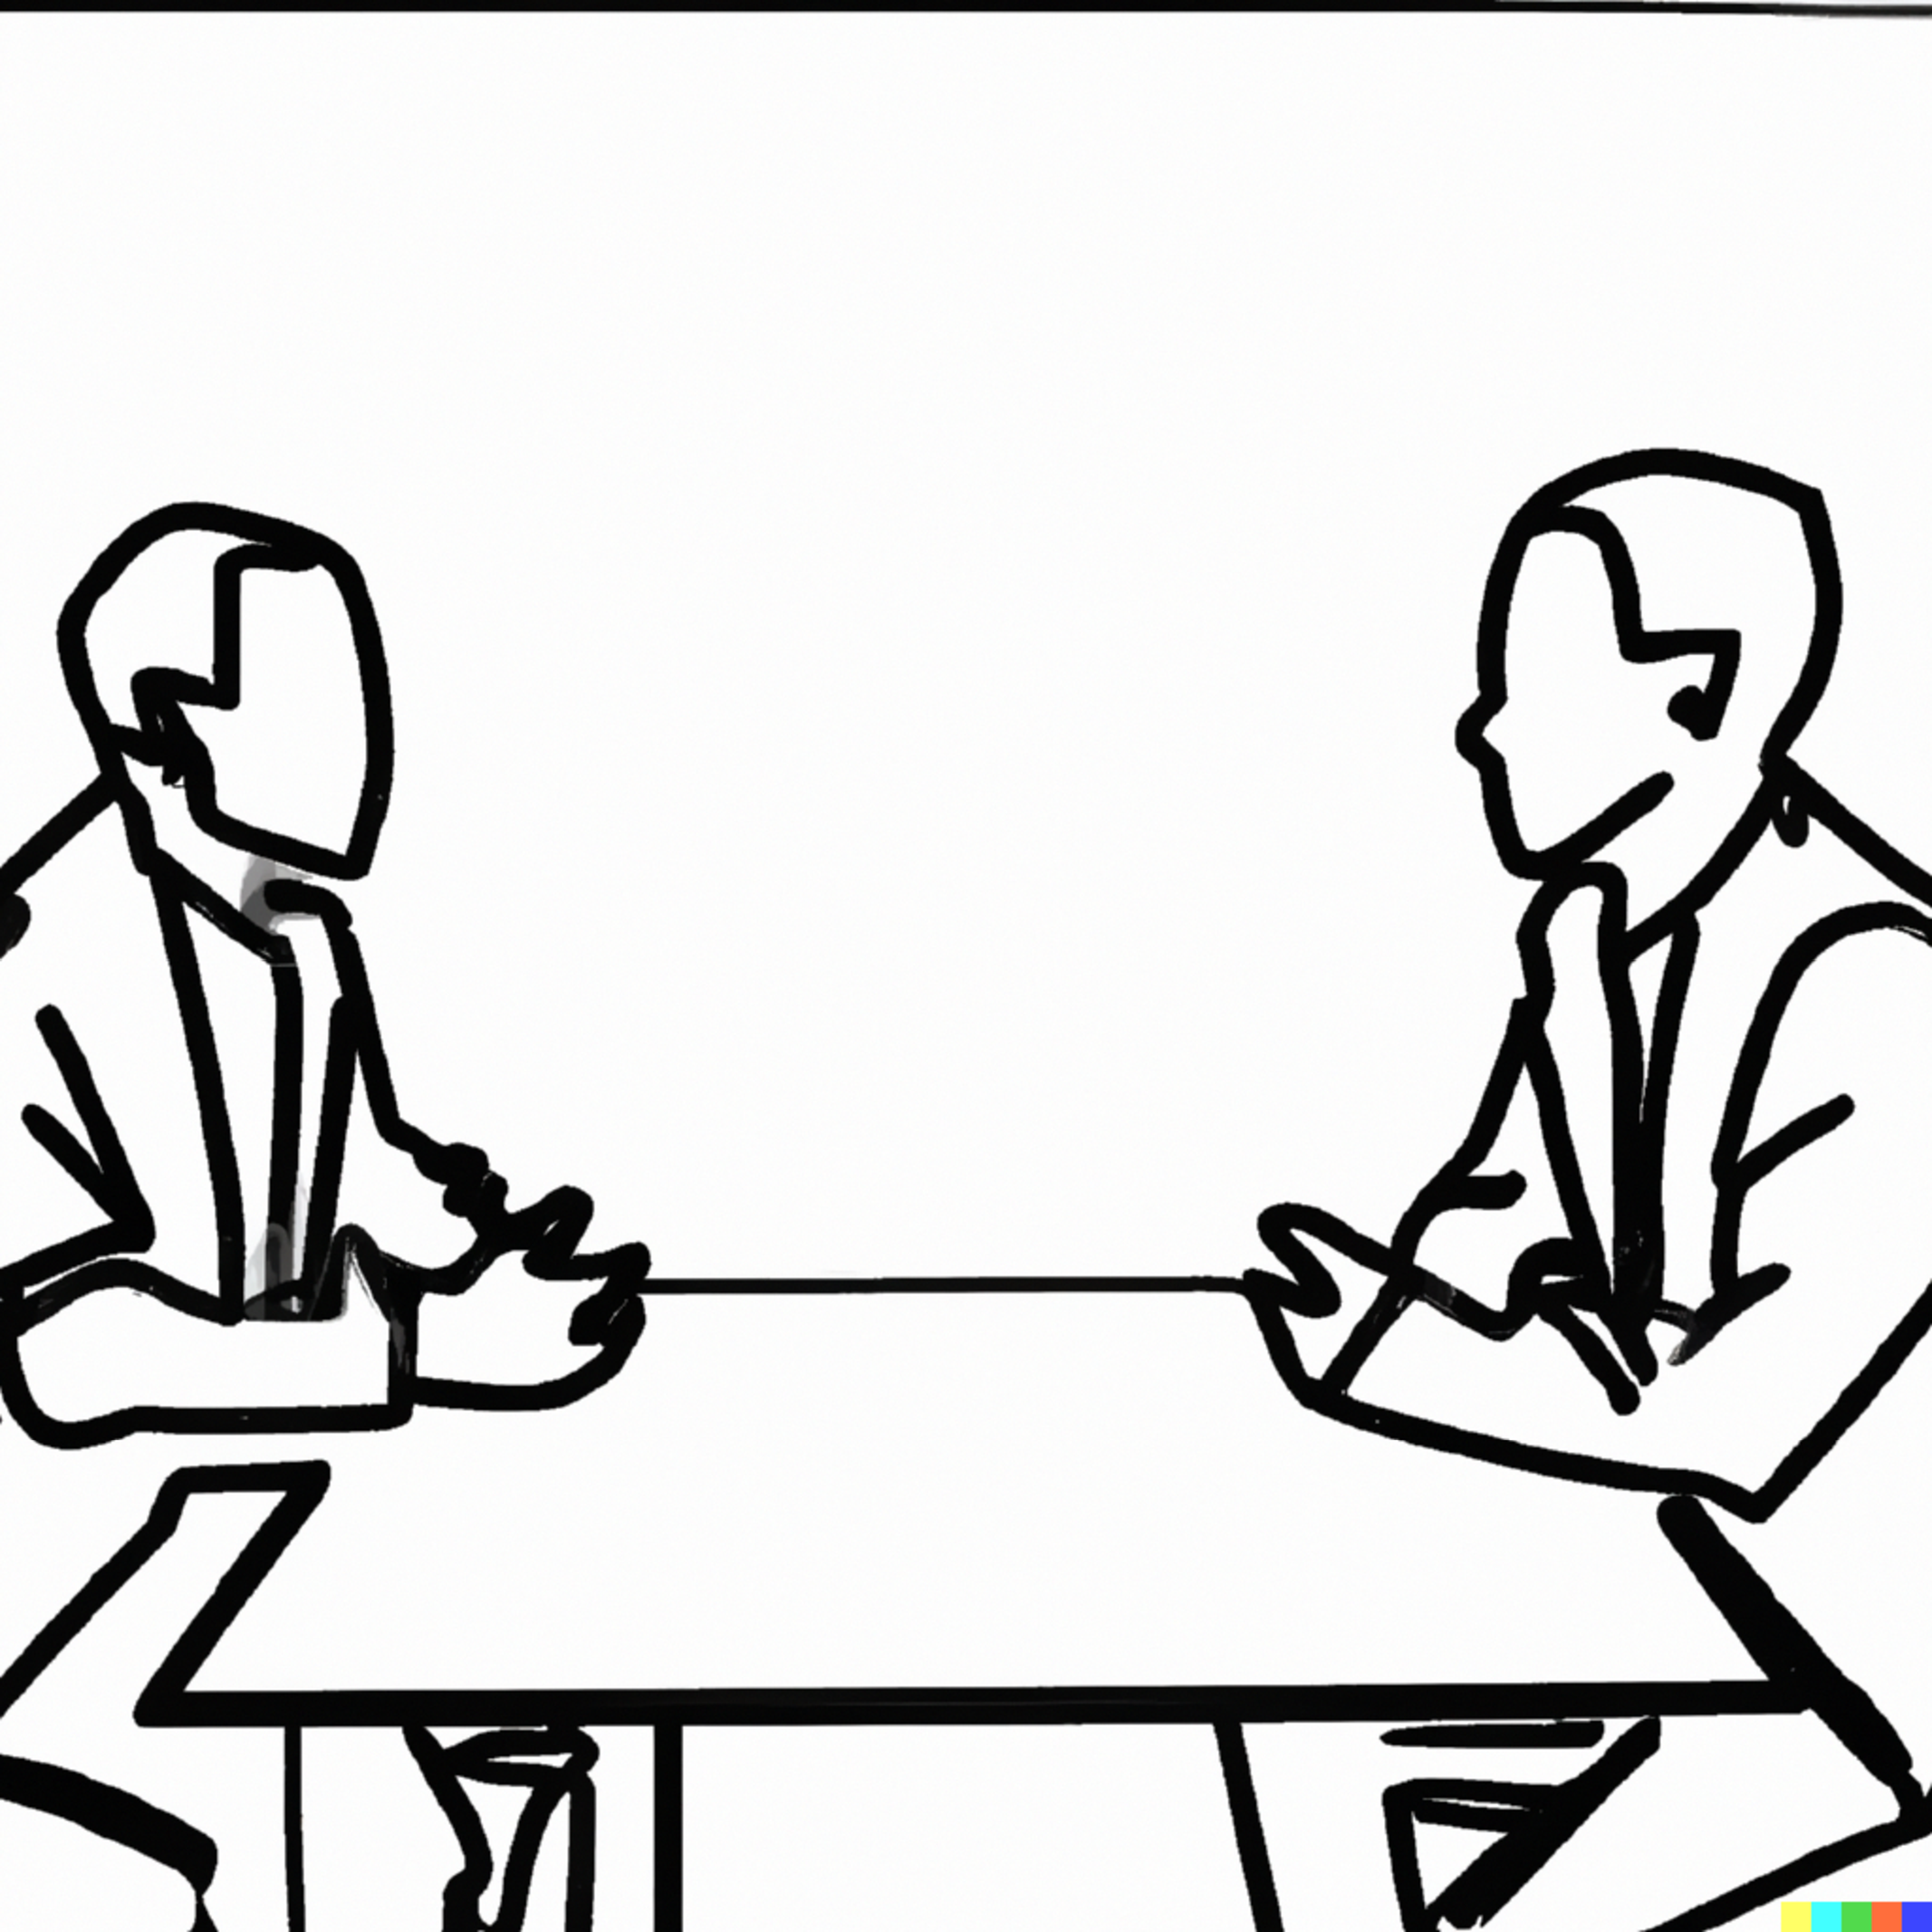
\includegraphics[width=0.6\textwidth]{images/confrontational_meeting_of_two_people_in_a_conference_room_both_are_seated.pdf}
    \caption{Meeting to discuss the value of coordination.}
    \label{fig:meeting-to-discuss-coordination}
\end{figure}


\ \\
\textit{Anti-meeting view}: What is a plan anyways?\\
\textit{Potential response by the supervisor}: There is value in collaboratively specifying a goal, enumerating tasks that would support the goal, identifying the dependencies among the sub-tasks, and time-binning the dependencies with defined milestones and deliverables. That is my definition of a plan. And having that is more useful than merely reacting.

\ \\
\textit{Anti-meeting view}: Who's plan? Who's relationships? I don't need to come up with that plan, the supervisor already has a plan. Just tell me what the plan is.\\
\textit{Potential response by the supervisor}: That's not as effective as coming up with independent plans and then resolving the differences. There's value in resolving the differences, even though that will cost time and frustration and displace time to enact the plan.


\ \\

Not every team member in a bureaucracy is against planning, or as obstinate about collaboration. 
My intent for sharing these debates is that you will be less surprised when they are raised by your coworkers. 
